\documentclass[conference, letterpaper]{IEEEtran}

\usepackage{listings}
\usepackage{graphicx}

\usepackage[cmex10]{amsmath}
\usepackage{color}
\usepackage{fancyhdr}
\usepackage[caption=false,font=footnotesize]{subfig}
\usepackage{tikz}
\usepackage{subfig}
\usepackage{multicol}

\usetikzlibrary{positioning,shapes,arrows}

\renewcommand{\thispagestyle}[2]{} 

\fancypagestyle{plain}{
        \fancyhead{}
        \fancyhead[C]{first page center header}
        \fancyfoot{}
        \fancyfoot[C]{first page center footer}
}
\pagestyle{fancy}


\headheight 31.99992pt
\footskip 20pt

\rhead{}

% First page number
\setcounter{page}{1}

% Header
\fancyhead[R]{\textit{
  RIT Computer Science ~\textbullet~ Capstone Report ~\textbullet~ 2215
}}
\renewcommand{\headrulewidth}{0pt}

% Footer
\fancyfoot[C]{Rochester Institute of Technology}
\renewcommand{\footrulewidth}{0.5pt}
\fancyfoot[R]{\thepage \  $|$ P a g e }


% Document starts here
\begin{document}

% Title
\title{Autonomous Navigation for Mobile Robots}

% Author
\author{\IEEEauthorblockN{Sagar Khadse}
\IEEEauthorblockA{
  Department of Computer Science\\
  Golisano College of Computing and Information Sciences\\
  Rochester Institute of Technology\\
  Rochester, NY 14586\\
  sk9877@rit.edu
}}

\maketitle

% Abstract
\begin{abstract}
The intent of this project was to develop an autonomous indoor navigation system
for mobile robots. The design involves a Pioneer 3-DX robot chassis with a 
Microsoft Kinect camera mounted on it. It was implemented using RTAB-Map, a 
graph-based SLAM approach that uses RGB and depth images from the Kinect camera.
This project adds a floor plan localization node that plots the position of the 
agent within a given floor plan of the building. The system was used to map the 
top floor of the RIT CS department and provide accurate localization for the 
robot within this map.
\end{abstract}

\begin{IEEEkeywords}
SLAM; Microsoft Kinect; Computer Vision; ROS
\end{IEEEkeywords}

\IEEEpeerreviewmaketitle

% Introduction
\section{Introduction}
Mobile Robots are developed for moving in known or unknown environments and 
performing a set of given tasks. These are especially helpful in industrial 
warehouses to move around goods efficiently and also in situations where it is 
unsafe for humans to operate. Making mobile robots autonomous allows the 
robots to perform repetitive tasks efficiently and without the need of 
individual control over each robot. Autonomous mobile robots need to be 
able to sense the environment and navigate through it. Primitive sensors such as
sonar or light proximity sensors can be used to navigate by avoiding obstacles 
but they are unaware of the environment until one of the sensors detects 
something. Knowing the environment before hand allows for more efficient path 
planning but this knowledge is not always available. To be able to intelligently
navigate the robot needs to be aware of its surroundings and it's location within
it. This can be achieved using Simultaneous Localization and Mapping (SLAM). 
SLAM algorithms take inputs from devices such as cameras and 2D Lidar to produce
a 2D or even 3D map of the surrounding while also keeping track of where the 
agent is in this map. 

Most SLAM algorithms generate maps and localize within them, they do not 
account for how these points corelate with the real world. We can find a 
corelation between the generated map and the floor plans of the building
to get true localization. This also allows for higher level path 
planning using known features of the building such as room numbers, 
floors and other landmarks that can be easily mapped on the floor plan.   
This project aims to implement such a SLAM approach on mobile robots for 
indoor navigation and improve localization by mapping the robot location 
on the real world floor plans of the building.

% Related Work
\section{Related Work}

\subsection{Comparison of Various SLAM Systems for Mobile Robot in an Indoor Environment}
This article presents a comparative analysis of a mobile robot trajectories computed by various ROS-based SLAM systems. For this reason we developed a prototype of a mobile robot with common sensors: 2D lidar, a monocular and ZED stereo cameras. Then we conducted experiments in a typical office environment and collected data from all sensors, running all tested SLAM systems based on the acquired dataset. We studied the following SLAM systems: (a) 2D lidar-based: GMapping, Hector SLAM, Cartographer; (b) monocular camera-based: Large Scale Direct monocular SLAM (LSD SLAM), ORB SLAM, Direct Sparse Odometry (DSO); and (c) stereo camera-based: ZEDfu, Real-Time Appearance-Based Mapping (RTAB map), ORB SLAM, Stereo Parallel Tracking and Mapping (S-PTAM). Since all SLAM methods were tested on the same dataset we compared results for different SLAM systems with appropriate metrics, demonstrating encouraging results for lidar-based Cartographer SLAM, Monocular ORB SLAM and Stereo RTAB Map methods.

\subsection{SLAM in indoor environments with stereo vision}
This paper proposes a method for simultaneous localisation and mapping (SLAM) in an indoor environment using stereo vision. Specially designed artificial landmarks distributed in the environment are observed and extracted from a camera image. The disparity map obtained from the stereo vision system is used to obtain the ranges to these landmarks. The main contribution of the paper is the formulation of the mathematical framework for SLAM for a robot moving on a planar surface among landmarks distributed in three dimensional space. The paper also presents the results of experiments conducted using a pioneer robot and a Triclops stereo vision system. It is demonstrated that accurate robot and feature locations can be obtained using the proposed technique.

\subsection{Simultaneous Localization and Mapping (SLAM) using RTAB-MAP}
This paper implements Simultaneous Localization and Mapping (SLAM) technique to construct a map of a given environment. A Real Time Appearance Based Mapping (RTAB-Map) approach was taken for accomplishing this task. Initially, a 2d occupancy grid and 3d octomap was created from a provided simulated environment. Next, a personal simulated environment was created for mapping as well. In this appearance based method, a process called Loop Closure is used to determine whether a robot has seen a location before or not. In this paper, it is seen that RTAB-Map is optimized for large scale and long term SLAM by using multiple strategies to allow for loop closure to be done in real time and the results depict that it can be an excellent solution for SLAM to develop robots that can map an environment in both 2d and 3d. 

\section{Hardware Specifications}
The mobile robot is built using the Pioneer 3-DX robot platform, it is a two 
wheel differential drive robot chassis with wheel encoders and 16 sonar sensors 
(8 front + 8 rear) for obstacle avoidance. It runs the ARCOS firmware supporting
the Pioneer protocol. For visual SLAM, the Microsoft Kinect camera is mounted open
top of the chassis. The Kinect is a combination of an RGB camera and a depth 
camera such a combination is also known as an RGB-D camera. The RGB camera 
captures images at 640 x 480 (30fps) while the depth camera captures images at 
320 x 240 (30fps) reliably up to a maximum depth of 4 meters. The compute 
platform is a laptop running Ubuntu (Linux) and ROS.

\begin{figure}[h]
  \centering
  \begin{tikzpicture}
    \node(robot){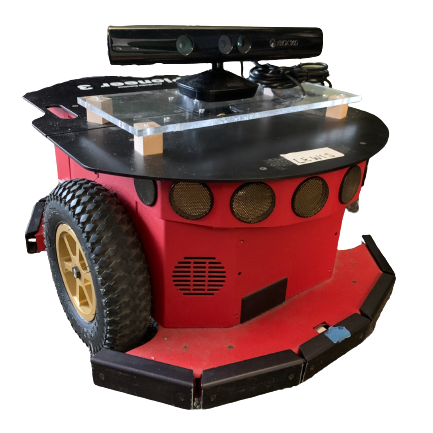
\includegraphics[width=0.6\linewidth]{assets/hardware.png}};
    \node(kinect) at (3.5,2.1){Microsoft Kinect};
    \node(pioneer) at (3.5,-0.5){Pioneer 3-DX};

    \draw[-stealth] (kinect) -- (1.5,2.1);
    \draw[-stealth] (pioneer) -- (1,-0.5);
  \end{tikzpicture}
  \caption{Mobile Robot Design}
\end{figure}

\section{System Design}

The navigation system is built using the Robot Operating System (ROS) framework.
ROS is a collection of software libraries that can be used to develop robotics 
systems. ROS uses a modularized approach to development where each function is 
a separate node and they use the publisher-subscriber model for communication. 
ROS provides message formats to encapsulate data from most sensors, this allows
a wide variety of sensors and devices from different manufacturers to 
communicate using a common protocol.

This system consists of four nodes namely \textit{freenect}, \textit{p2os}, 
\textit{rtabmap\_ros} and \textit{floor\_localization}.

\subsection{Freenect}

Freenect (libfreenect) is an open-source driver for the Microsoft Kinect. It
provides functions to access the RGB camera, depth camera, motors, 
accelerometer and microphone array present on the Kinect. The driver can be 
used to capture RGB and depth images from the camera. To be able to 
communicate in ROS, we use \emph{freenect\_camera} package which is a 
libfreenect-based ROS driver for the Microsoft Kinect. The topics of interest 
for this project are as follows,
\begin{itemize}
  \item \textbf{/rgb/camera\_info:} Camera calibration data
  \item \textbf{/rgb/image\_raw:} Raw RGB image
  \item \textbf{/depth\_registered/image\_raw:} Raw depth image
\end{itemize}

\begin{figure}[ht]
  \centering
  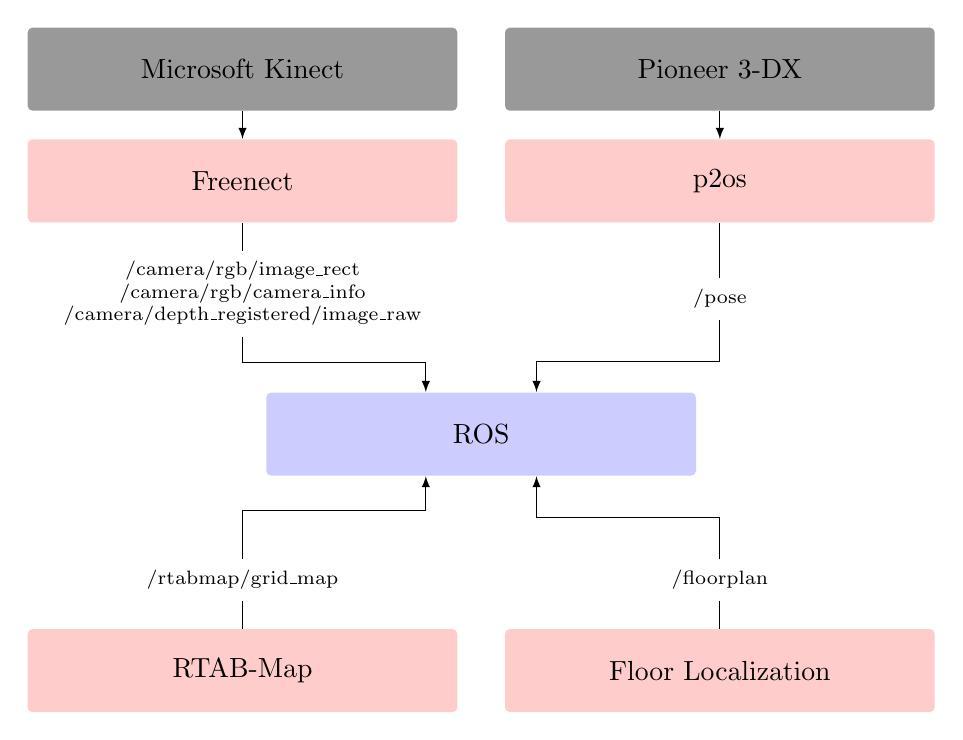
\begin{tikzpicture}[
    block/.style={ 
      rounded corners=0.4ex, fill=black!20, text centered, inner sep=2ex, 
      minimum height=3em, minimum width=6em
    },
    full/.style={block, minimum width=0.95\linewidth},
    half/.style={block, minimum width=0.45\linewidth},
    node/.style={fill=red!20},
    core/.style={fill=blue!20},
    device/.style={fill=black!40},
  ]
    \node[half, device](kinect) at (-0.25\linewidth, 0) {Microsoft Kinect};
    \node[half, node, below=1em of kinect](freenect){Freenect};
    \node[below=1em of freenect](freenect_pub){
      \scriptsize
      \begin{tabular}{c}
        /camera/rgb/image\_rect \\
        /camera/rgb/camera\_info \\
        /camera/depth\_registered/image\_raw \\
      \end{tabular}
    };
    
    \node[half, device](robot) at (0.25\linewidth, 0) {Pioneer 3-DX};
    \node[half, node, below=1em of robot](p2os){p2os};
    \node[below=2em of p2os](p2os_pub){
      \scriptsize
      \begin{tabular}{c}
        /pose
      \end{tabular}
    };
    
    \node[half, core, below=2em of freenect_pub, xshift=0.25\linewidth](ros){ROS};

    \node[below=3em of ros, xshift=-0.25\linewidth](rtabmap_pub){
      \scriptsize
      \begin{tabular}{c}
        /rtabmap/grid\_map
      \end{tabular}
    };
    \node[half, node, below=1em of rtabmap_pub](rtabmap){RTAB-Map};

    \node[below=3em of ros, xshift=0.25\linewidth](loc_pub){
      \scriptsize
      \begin{tabular}{c}
        /floorplan
      \end{tabular}
    };
    \node[half, node, below=1em of loc_pub](loc){Floor Localization};
    
    \draw[-latex] (kinect) -- (freenect);
    \draw[-latex] (robot) -- (p2os);
    \draw[-] (freenect) -- (freenect_pub);
    \draw[-latex] (freenect_pub) |- +(2em,-2.5em) -| ([xshift=-2em]ros.north);
    \draw[-] (p2os) -- (p2os_pub);
    \draw[-latex] (p2os_pub) |- +(-2em,-2.25em) -| ([xshift=2em]ros.north);
    \draw[-] (rtabmap) -- (rtabmap_pub);
    \draw[-latex] (rtabmap_pub) |- +(2em,2.5em) -| ([xshift=-2em]ros.south);
    \draw[-] (loc) -- (loc_pub);
    \draw[-latex] (loc_pub) |- +(-2em,2.25em) -| ([xshift=2em]ros.south);
    
  \end{tikzpicture}
  \caption{System Overview}

\end{figure}

\subsection{p2os}

p2os is a ROS driver for robots using the P2OS, AROS or ARCOS firmware and 
Pioneer protocol. The driver provides support for running robot motors using 
velocity control and publishes the state of the robot and its sensors.
The topics of interest for this project are as follows,
\begin{itemize}
  \item \textbf{/pose:} Robot pose data
  \item \textbf{/tf:} Reference coordinate frame and robot position frame
\end{itemize}

\subsection{RTAB-Map}

RTAB-Map (Real-Time Appearance-Based Mapping) is a graph-based SLAM approach 
that uses appearance-based loop closure detection. This package supports 
implementing visual or lidar-based SLAM using a variety of hardware including
Lidar, Stereo cameras and RGB-D cameras. The package includes modules for 
robust visual odometry using the supported camera configurations along with 
support for using wheel odometry data directly from the robot. A few example
configurations are listed below,

\begin{itemize}
  \item Kinect
  \item Kinect + 2D laser
  \item Kinect + Odometry
  \item Kinect + Odometry + 2D laser
  \item Kinect + Odometry + Fake 2D laser from Kinect
\end{itemize}

Loop closure is performed using the bag-of-words approach where visual features
extracted from the RGB image are used to build an incremental visual word 
vocabulary, features from new images are matched against these to identify 
potential loop closure. When a loop closure is detected the graph is optimized 
to minimize the errors in the map. 

RTAB-Map provides a large number of parameters to fine-tune the functioning of 
the module based on requirement. It also supports a Multi-session mapping mode 
to allow mapping smaller areas and combining them to produce a larger map, this 
is especially helpful for covering larger areas using robots with onboard 
batteries. 

\subsection{Floor Localization}

SLAM algorithms generate a 2D or 3D occupancy grid map that is later used for 
localization but this does not provide corelation with the real world. For such 
a corelation we need information about the building and need to manually 
annotate the generated map. Instead it is possible to extract this information
from the floor plans of the mapped area. Floor plans are extensively detailed 
and can be very helpful for the user to easily identify with.

\begin{figure}[ht]
  \centering
  \subfloat[Floor Plan]{
    \includegraphics[width=0.45\linewidth]{assets/f4_a.png}  
  }
  \hfill
  \subfloat[Corridor Binary Mask]{
    \includegraphics[width=0.45\linewidth]{assets/f4_b.png}  
  }
  \hfill
  \subfloat[2D Occupancy Grid]{
    \includegraphics[width=0.45\linewidth]{assets/f4_c.png}  
  }
  \hfill
  \subfloat[Occupancy Mask]{
    \includegraphics[width=0.45\linewidth]{assets/f4_d.jpg}  
  }
  \hfill
  \subfloat[Template Matching]{
    \includegraphics[width=0.45\linewidth]{assets/f4_e.jpg}  
  }
  \caption{Floor Localization Working}  
\end{figure}

The floor localization module creates a boolean mask from the floor plan of the 
area and tries to align it with the generated 2D Occupancy grid. As a result we 
get a transformation of the points on the generated map to the floor plan. The 
position of the agent can then be plotted onto the floor plan allowing the use 
of more real world landmarks such as rooms for efficient path planning.

\section{Experiments}

A number of experiments with varying hardware and software combinations were 
performed in order to determine the best fit for this application. Some of them 
are explained in the following sections for better understanding of the process 
of tuning the system for a specific application.

\subsection{Mapping with a Handheld Kinect}

The first experiment involved mapping a single room using a handheld Kinect 
camera used in combination with RTAB-Map to create a 3D map. Since RTAB-Map 
supports Kinect out of the box, there was no additional configuration required
and one of the sample launch files provided was used. 

\begin{figure}[ht]
  \centering
  \subfloat[Feature Rich Environment]{
    
\includegraphics[width=0.45\linewidth]{assets/placeholder.png}  
  }
  \hfill
  \subfloat[Low Feature Environment]{
    
\includegraphics[width=0.45\linewidth]{assets/placeholder.png}  
  }
  \caption{Handheld Kinect Mapping Issues}  
\end{figure}

When using the Kinect as the only input to RTAB-Map, the odometry needed to be 
computed by tracking the motion between consecutive frames. To achieve this, 
RTAB-Map uses a visual odometry approach that relies on extracting visual 
features such as SIFT, SURF and ORB and matching them in consecutive frames to 
predict the motion of the camera. This approach works in feature-rich 
environments (see fig1) but fails when there are few or no features to track in 
the image, for example blank walls (see fig2). Losing track implies that the 
motion of the camera can no longer be tracked reliably, causing a failure in the 
mapping process.

\subsection{Kinect mounted on Robot Chassis}

Visual odometry is not reliable when used in low feature environments as seen in 
the previous section, there is a need for a more reliable source of odometry. 
The Pioneer 3-DX is a robot platform that has wheel encoders and is compatible 
with ROS. Mounting the camera onto the robot chassis allowed the use of odometry 
data from the robot chassis along with the images from the camera to improve 
tracking. The odometry from the robot was not only more reliable but also 
smoother compared to the jagged path produced by visual odometry. The new setup 
produced better results when mapping the same room.

\begin{figure}[ht]
  \centering
  \subfloat[Visual Odometry]{
    \includegraphics[width=0.45\linewidth]{assets/f5_a_visual.png}  
  }
  \hfill
  \subfloat[Wheel Odometry]{
    \includegraphics[width=0.45\linewidth]{assets/f5_b_wheel.png}  
  }
  
  \hfill
  \subfloat[Mapping with Visual Odometry]{
    \includegraphics[width=0.45\linewidth]{assets/f4_c_mapping_error.png}  
  }
  \hfill
  \subfloat[Mapping with Wheel Odometry]{
    \includegraphics[width=0.45\linewidth]{assets/f5_c_wheel_map.png}  
  }
  \caption{Improvements using Wheel Odometry}  
\end{figure}

\subsection{Mapping a Larger Area}

Mapping a selected section of the floor using the current configuration 
identified issues with the wheel odometry data. When mapping a smaller area like
a room, errors in mapping were smaller and unnoticeable. Over larger distances, 
it was observed that the wheel odometry isn't perfect and the error accumulated 
over time causing a drift from the actual path of the robot. To mitigate this 
issue RTAB-Map uses loop closure to identify potential loops and optimize the 
map to correct errors. The area used for mapping consisted of large corridors 
that are visually very similar, this caused the rtabmap to perform incorrect 
loop closures and reject correct ones.

\begin{figure}[ht]
  \centering
    \includegraphics[width=\linewidth]{assets/f6_similarities.png} 
  \caption{Similarities in images at different locations}  
\end{figure}

Looking at the images it was identified that the floor and ceiling in the 
images were almost identical in different locations and most of the detail lay 
in the central portion of the image. The region of interest for loop closure was
set the the central third of the image for more distinguishable feature 
extraction. Mapping using the new region of interest configured worked for 
correcting smaller drifts but wasn't able to correct larger errors accumulated 
over longer paths. The loop closures were being rejected by RTAB-Map due to 
large errors, increasing the rejection threshold fixed these issues.

\begin{figure}[ht]
  \centering
  \subfloat[]{
    \includegraphics[width=0.45\linewidth]{assets/f7_a.png}  
  }
  \hfill
  \subfloat[]{
    \includegraphics[width=0.45\linewidth]{assets/f7_b.png}  
  }
  \caption{Loop Closure Tuning}  
\end{figure}

When taking a larger loop, the drift in the odometry accumulates to such an 
extent that the loop closure detector is unable to identify the locations being
the same. The robot odometry was biased towards the right causing straight paths
to bend towards the right. Moving the robot in smaller loops causes closing 
loops earlier and reduces the accumulated error.

\begin{figure}[ht]
  \centering
  \includegraphics[width=0.6\linewidth]{assets/f8_large_loop.png}  
  \caption{Accumulated Error for Large Loop}  
\end{figure}  

\begin{figure*}[!t]
  \centering
  \subfloat[Floor Plan]{
    \includegraphics[width=0.9\textwidth]{assets/f8_a_mapped_area.png}  
  }
  \hfill
  \subfloat[3D Point Cloud]{
    \includegraphics[width=0.9\textwidth]{assets/f8_b_2d_occupancy.png}  
  }
  \hfill
  \subfloat[2D Occupancy Grid]{
    \includegraphics[width=0.9\textwidth]{assets/f8_b_2d_occupancy.png}  
  }
  \caption{Mapping Results}  
\end{figure*}  


\newpage

\section{Mapping}

The main corridor of the 3rd floor of the RIT CS department was mapped using the 
robot. The mapping was performed across multiple sessions of mapping smaller 
areas at a time due to battery constraints. During the mapping process, it was 
observed that moving through the same location multiple times improved the 
overall accuracy of the map. 

% Conclusion
\section{Conclusion}

The main corridor of the 3rd floor of the RIT CS department was mapped using the 
robot. The mapping was performed across multiple sessions of mapping smaller 
areas at a time due to battery constraints. During the mapping process, it was 
observed that moving through the same location multiple times improved the 
overall accuracy of the map.

% References
\nocite{*}
\bibliographystyle{IEEEtran}
\bibliography{IEEEabrv,report}

\end{document}


